\documentclass[wide,a4paper,titlepage,12pt]{mwart}
\usepackage{polski,graphicx,pdflscape}
\usepackage[utf8]{inputenc}
\usepackage{listings}


\title{Autokorelacja i korelacja wzajemna}
\author{Tymon Tobolski (181037)\\ Jacek Wieczorek (181043)}

% Title page layout (fold)
\makeatletter
\renewcommand{\maketitle}{
\begin{titlepage}
  \begin{center}
    \vspace*{3cm}
    \LARGE \@title \par
    \vspace{2cm}
    \textit{\small Autor:}\par
    \normalsize \@author\par \normalsize
    \vspace{3cm}
    \textit{\small Prowadzący:}\par
    Dr inż. Paweł Biernacki \par
    \vspace{2cm}
    Wydział Elektroniki\\ II rok\\ WT/TN 13:15--15:00 \par
    \vspace{5cm}
    \small \@date
  \end{center}
\end{titlepage}
}
\makeatother
% Title page layout (end)

\begin{document}
  \maketitle
  \section{Cel ćwiczenia} % (fold)
  \label{sec:Cel}
    Zbadanie przebiegu funkcji autokorelacji i korelacji wzajemnej dla różnych typów sygnałów.
    
  \section{Algorytm przetwarzający}
    Wykorzystane funkcje:
    \newline
    \begin{itemize}
      \item generujące sygnał (\textbf{sinus}, \textbf{prostokat}, \textbf{randn})
      \item obliczające korelacje (\textbf{xcorr})
    \end{itemize}
  
  \lstset{ %
    language=Octave,                % choose the language of the code
    basicstyle=\scriptsize,       % the size of the fonts that are used for the code
    numbers=left,                   % where to put the line-numbers
    numberstyle=\scriptsize,      % the size of the fonts that are used for the line-numbers
    stepnumber=10,                   % the step between two line-numbers. If it's 1 each line 
                                    % will be numbered
    numbersep=9pt,                  % how far the line-numbers are from the code
    % backgroundcolor=\color{white},  % choose the background color. You must add \usepackage{color}
    showspaces=false,               % show spaces adding particular underscores
    showstringspaces=false,         % underline spaces within strings
    showtabs=false,                 % show tabs within strings adding particular underscores
    % frame=single,                 % adds a frame around the code
    % tabsize=2,                  % sets default tabsize to 2 spaces
    % captionpos=b,                   % sets the caption-position to bottom
    breaklines=true,                % sets automatic line breaking
    % breakatwhitespace=false,        % sets if automatic breaks should only happen at whitespace
    % title=\lstname,                 % show the filename of files included with \lstinputlisting;
                                    % also try caption instead of title
    % escapeinside={\%*}{*)},         % if you want to add a comment within your code
    % morekeywords={*,...}            % if you want to add more keywords to the set
    }
    \lstinputlisting{lab2.m}
    
  % section Wstęp (end)
  
  \section{Autokorelacja}
	  \subsection{Sygnał sinus}
		\label{auto_sin}
		Badany sygnał został określony następującymi parametrami:
		
		$A=1, f=4, fpr=200, faza=0, T=2$
				
		Funkcja autokorelacji osiąga największą wartość, dla przesunięcia równego zero. oraz najmniejszą dla przesunięcia $\pi$ i $\-pi$. Wykres funkcji corr. jest symetryczny względem osi y. i w danych przedziałach przyjmuje wartość największą gdy przesunięcie jest całkowitą wielokrotnością $2\pi$, najmniejszą dla całkowitej wielokrotności $\pi$, a zero dla przesunięcia $\frac{\pi}{2}$.
		
      	Wykresy znajdują się na stronie \pageref{wykres1}.

	  \subsection{Sygnał cosinus}
		\label{auto_cos}
		Badany sygnał został określony następującymi parametrami:
		
		$A=1, f=4, fpr=200, faza=0, T=2$
		
		Wykres funkcji autokorelacji funkcji cosinus, jest identyczny jak wykres korelacji funkcji sinus. Dzieje się to dlatego, że funkcja cosinus jest taką samą funkcją okresową jak sinus, tylko przesuniętą o $\frac{\pi}{2}$.
		
		Wykresy znajdują się na stronie \pageref{wykres1}.

	  \subsection{Sygnał prostokątny}
	  \label{auto_prostokat}
		Sygnał prostokątny został określony parametrami:
		
		$A=1, f=4, fpr=200, faza=0, T=2, \omega$
		
		Funkcja autokorelacji została zbadana dla wartości wypełnienia $\omega \in \left \{0.1, 0.5, 0.9\right \}$
		
		Wraz ze wzrostem wypełnienia sygnału prostokątnego, funkcja korelancji przyjmuje mniej wartości zerowych, ponieważ, zmniejszają się przedziały okresu sygnału, w którym przyjmuje wartość zero. Wartość maksymalną przyjmuje dla przesunięcia równego zero.
				
		Wykresy znajdują się na stronach \pageref{wykres2} i \pageref{wykres3}.
		
	  \subsection{Szum biały}
		Szum biały jest generowany na podstawie funkcji \textbf{randn}, opartej o rozkład normalny. Maksymalną wartość, znacznie większą od pozostałych, funkcja przyjmuje dla 0 przesunięcia. W poszostałych przypadkach wartości funkcji oscylują wokół wartości zero.
		
    	Wykresy znajdują się na stronie \pageref{wykres2}.
		
		
  \section{Korelacja wzajemna}
	 \subsection{Sygnały sinus i cosinus}	
	 \label{cor_sin_cos}
		Wykorzystane zostały sygnały o identycznych parametrach jak w punktach \ref{auto_sin} oraz \ref{auto_cos}.
		
		Korelacja sygnałów sinusoidalnego i cosinusoidalnego przyjmuje wartość największą dla przesunięcia $\frac{\pi}{2}$ i najmniejszą dla przesunięcia  $-\frac{\pi}{2}$. Wykres funkcji nie jest symetryczny względem żadnej osi układu współrzędnych.
		
	 	Wykresy znajdują się na stronie \pageref{wykres4}.
	
	\subsection{Sygnały cosinus i sinus}
		Korelacja cosinus i sinus stanowi lustrzane odbicie funkcji korelacji dla sinusa i cosinusa (opisanej w punkcie \ref{cor_sin_cos}).
		
	 	Wykresy znajdują się na stronie \pageref{wykres4}.
	

	 \subsection{Sygnały sinus i prostokątny}	
		Wykorzystany został sygnał sinus o parametrach jak w punkcie \ref{auto_sin} oraz sygnał prostokątny o parametrach jak w punkcie \ref{auto_prostokat} i wypełnieniu $\omega=0.5$
		
		Funkcja korelacji wzajemnej osiąga maksymalną wartość dla zerowego przesunięcia, a minimalną dla przesunięcia równego połowie okresu sygnału prostokątnego. Wykres funkcji jest symetryczny względem środka układu współrzędnych.
					
		Wykresy znajdują się na stronie \pageref{wykres5}.
		
	 \subsection{Sygnały sinus i szum biały}	
		Wykorzystany został sygnał sinus o parametrach jak w punkcie \ref{auto_sin} oraz szum biały.

		Funkcja korelacji jest nieregularna, przyjmuje różne wartośći dla różnych przesunięć, nie tworzące żadnych regularnośći.

		Wykresy znajdują się na stronie \pageref{wykres5}.
	 	
 
      \begin{landscape}
        \begin{figure}[htbp]
          \begin{center}
            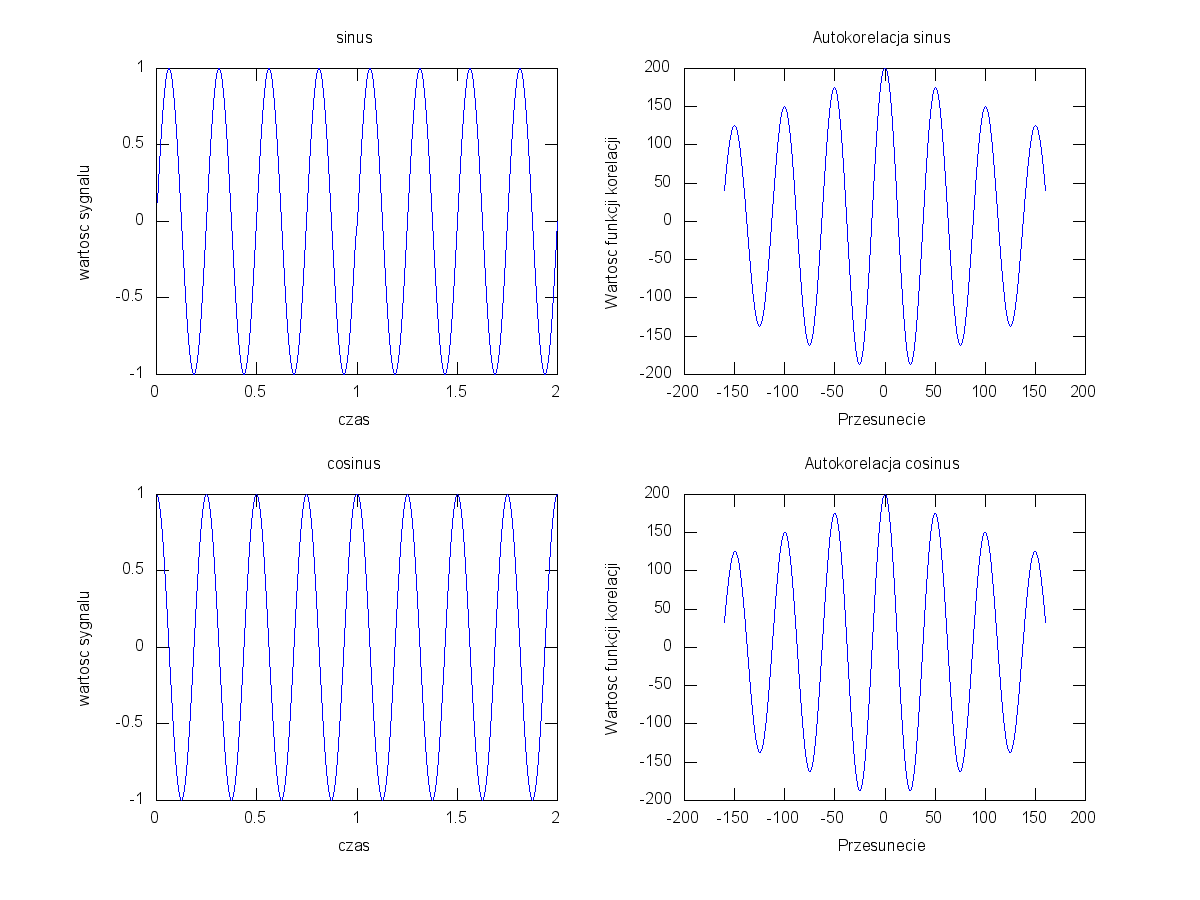
\includegraphics[scale=.5]{out/Figure1.png}
            \caption{\label{wykres1} Autokorelacja sinus i cosinus}
          \end{center}
        \end{figure}
      \end{landscape}

      \begin{landscape}
        \begin{figure}[htbp]
          \begin{center}
            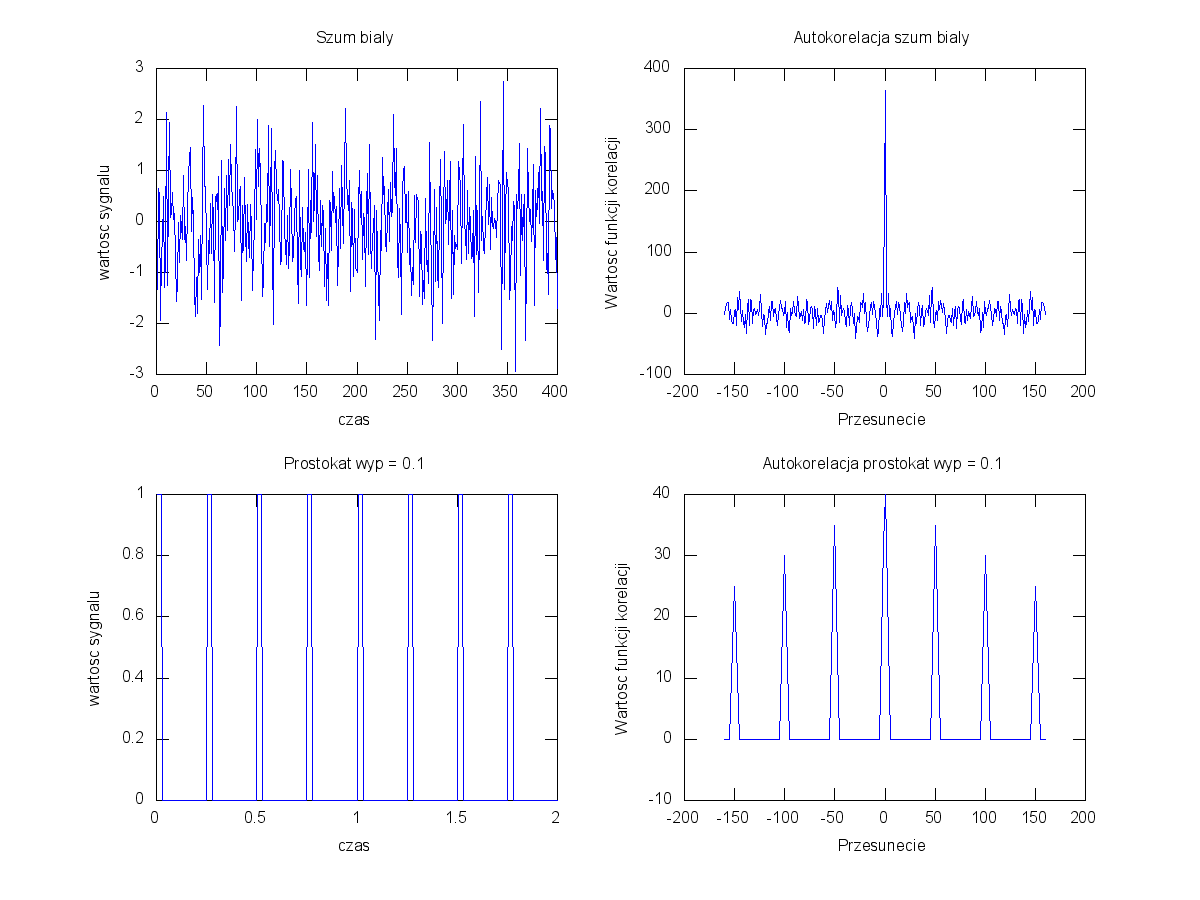
\includegraphics[scale=.5]{out/Figure2.png}
            \caption{\label{wykres2} Autokorelacja szumu białego i sygnału prostokątnego}
          \end{center}
        \end{figure}
      \end{landscape}

      \begin{landscape}
        \begin{figure}[htbp]
          \begin{center}
            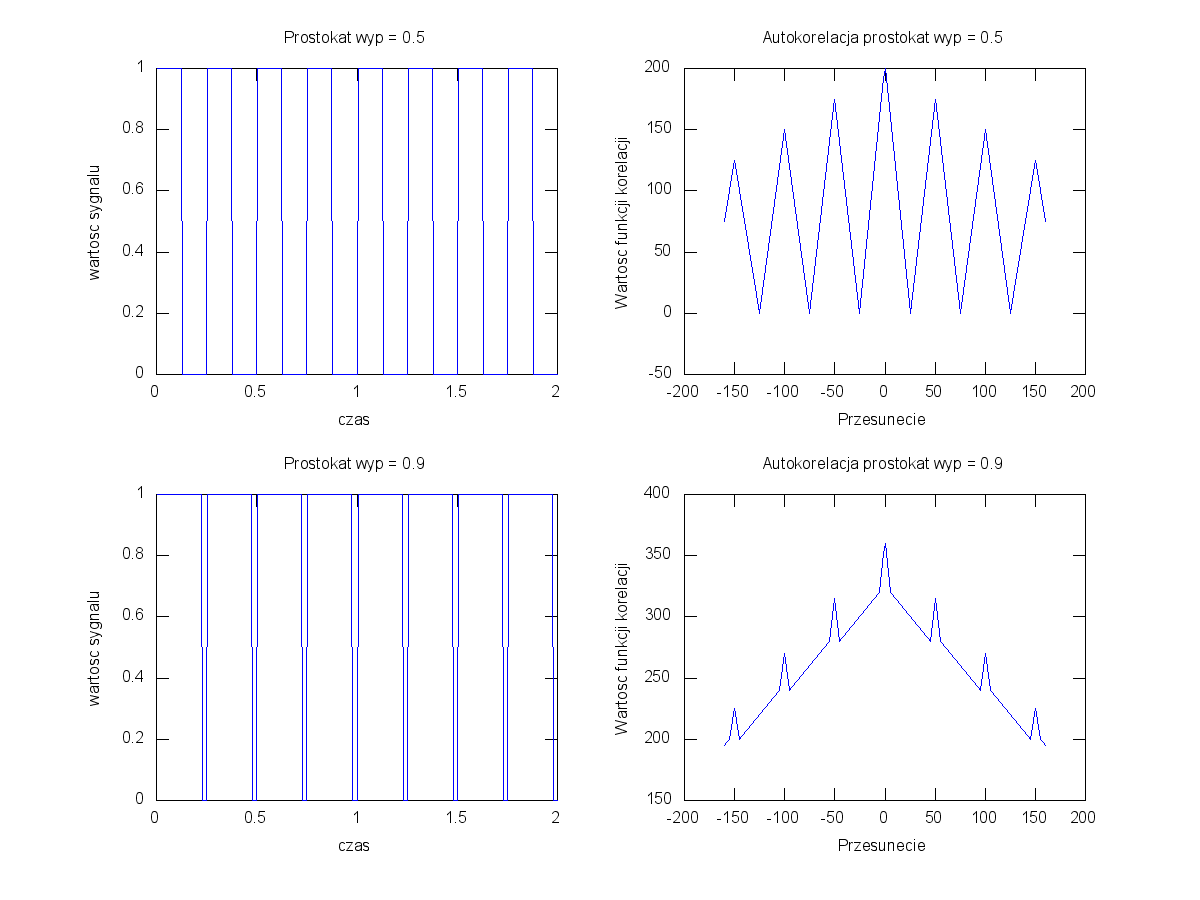
\includegraphics[scale=.5]{out/Figure3.png}
            \caption{\label{wykres3} Autokorelacja sygnału prostokątnego c.d.}
          \end{center}
        \end{figure}
      \end{landscape}

      \begin{landscape}
        \begin{figure}[htbp]
          \begin{center}
            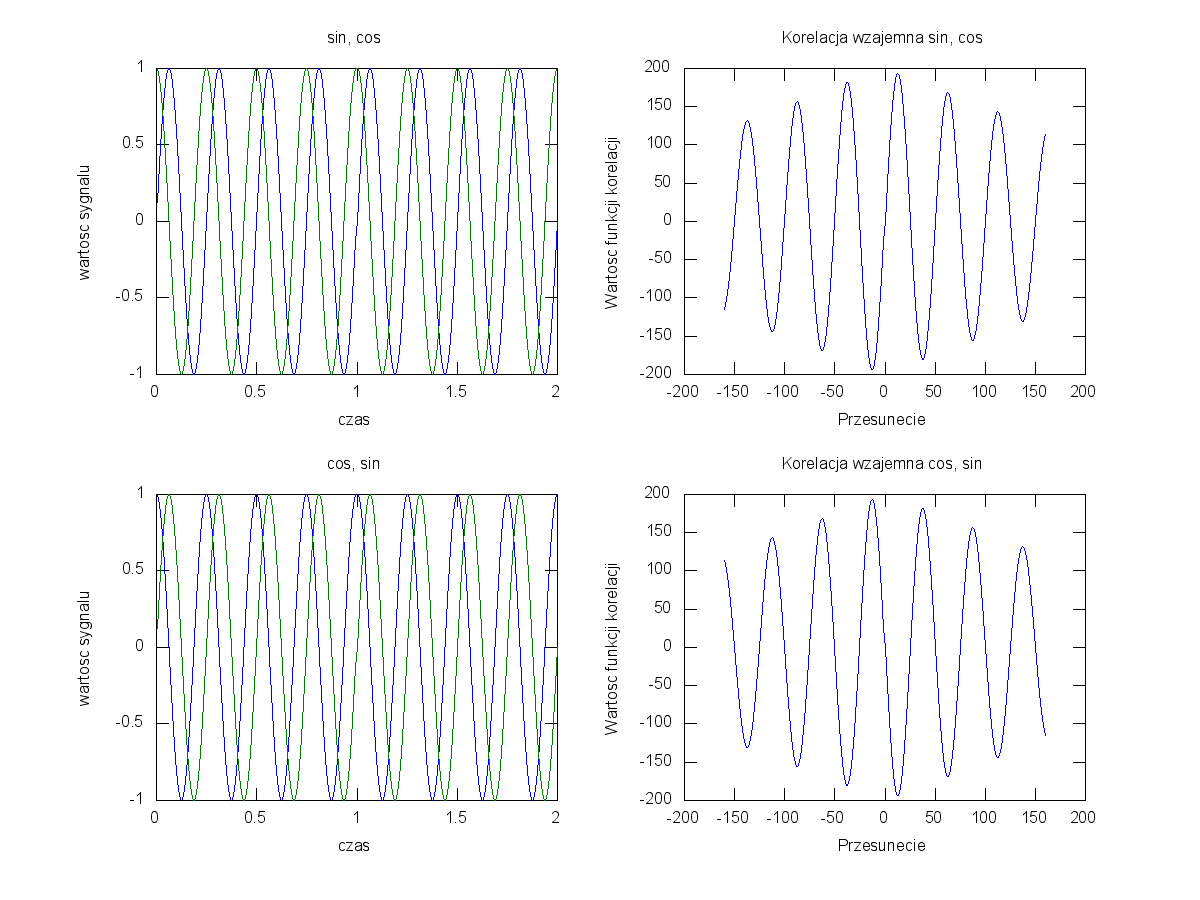
\includegraphics[scale=.5]{out/Figure4.png}
            \caption{\label{wykres4} Korelacja wzajemna sinus i cosinus oraz cosinus i sinus}
          \end{center}
        \end{figure}
      \end{landscape}

      \begin{landscape}
        \begin{figure}[htbp]
          \begin{center}
            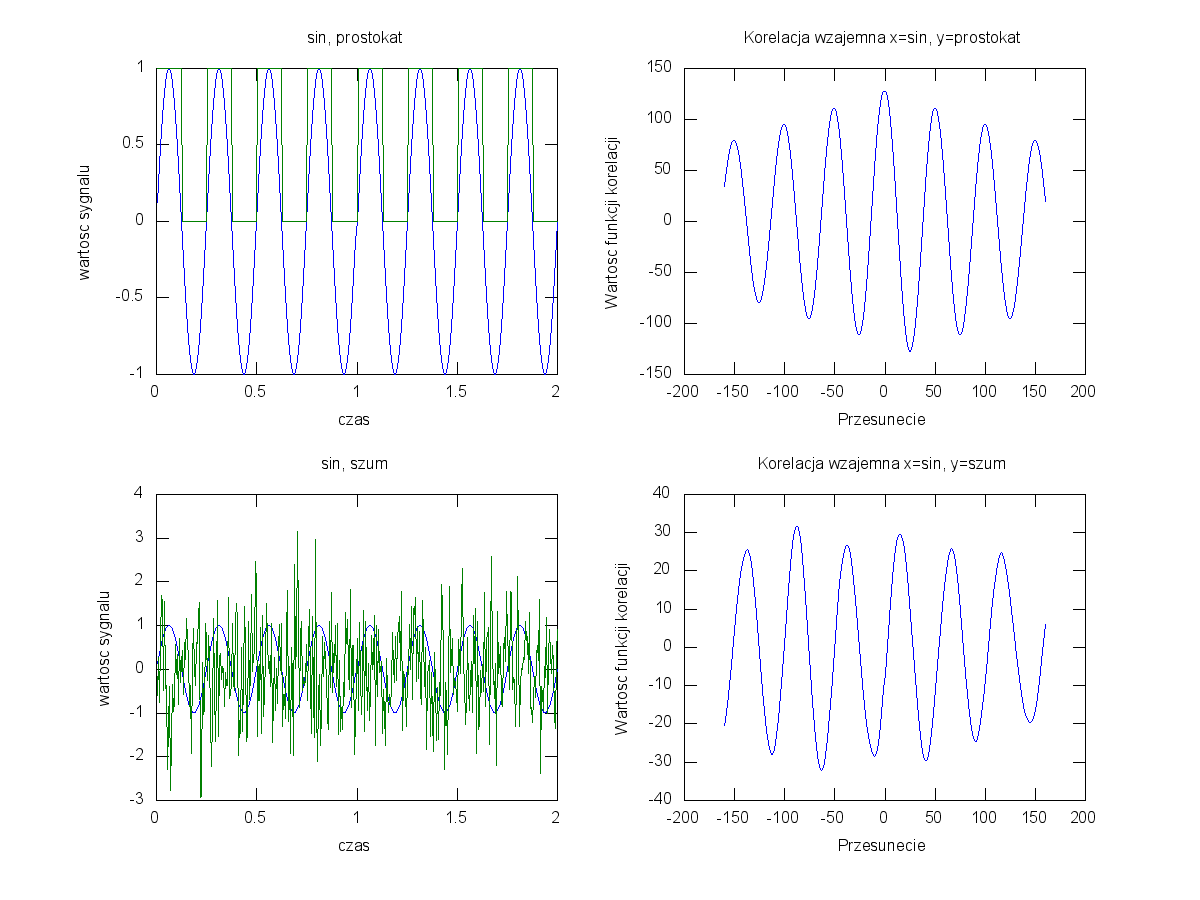
\includegraphics[scale=.5]{out/Figure5.png}
            \caption{\label{wykres5} Korelacja wzajemna: sinus i sygnał prostokątny oraz sinus i szum biały}
          \end{center}
        \end{figure}
      \end{landscape}
  
% Wykresy (end)
\end{document}